\documentclass[ignorenonframetext]{beamer}
%\documentclass[a4paper,12pt,titlepage]{article}
%\usepackage{beamerarticle}

\mode<article>{\usepackage[a4paper, top=1.5in]{geometry}}
%\mode<article>{\usepackage{fullpage}}
\mode<presentation>{\usetheme{JuanLesPins}}
%\usepackage{sansmathaccent}
%\pdfmapfile{+sansmathaccent.map}

%\includeonlylecture{Lecture 5}
%\includeonlyframes{current}

\AtBeginLecture{\frame{\Large \insertlecture}}

\logo{\includegraphics[height=1cm]{../graphics/crac.jpg}}
\usepackage{graphicx}
\usepackage{tikz}
\usepackage{pdfpages}
\usepackage{textcomp}
\usepackage{fancyhdr,url}
\usepackage{ulem}
\usepackage{bbm}
%\usepackage[dvipsnames]{xcolor}
\setlength{\parindent}{0in}

\mode<presentation>{\usepackage[absolute,overlay]{textpos}}
\mode<article>{\usepackage[absolute]{textpos} }

\mode<article>{
%\pagestyle{headings}

\pagestyle{fancy}
\fancyhf{}
\lhead{CM3017}
\chead{PHYSICAL CHEMISTRY 2}
\rhead{S1 2022-2023}
\lfoot{Stig Hellebust}
\cfoot{STATISTICAL THERMODYNAMICS}
\rfoot{\thepage}
}

\title{CM3017 -- Physical Chemistry 2}
\mode<presentation>{\subtitle{Introduction to Statistical Thermodynamics}\author{Stig Hellebust}
\institute{School of Chemistry \\ University College Cork}}
\mode<article>{\subtitle{Introduction to Statistical Thermodynamics\\\tiny{Version 2022.01}\\\vspace{1cm}
\includegraphics[height=1.5in]{../graphics/Boltzmann}\\
School of Chemistry, University College Cork}
}
\date{Semester 1 2022/2023}

\renewcommand*\contentsname{}

\begin{document}

\mode<article>{\maketitle}
\begin{frame}
	\titlepage
\end{frame}

\tableofcontents

\lecture{What is statistical thermodynamics}{Lecture 1}
\section{What is statistical thermodynamics}

\begin{frame}
What are the \underline{statistical population}, the \underline{configuration} and the \underline{weight}?
\end{frame}

\begin{frame}[allowframebreaks]
\frametitle{What is statistical thermodynamics?}
We know about energies that molecules can possess. \newline

Knowing is VERY important, because all energy contributes to the internal energy of the molecule, U\newline

We can demonstrat the existence of this kind og `partitioning' of energy in molecules using spectroscopy, but how does it relate to thermodynamics? \newline

Answer: quantum mechanics deals with the properties of individual molecules, while thermodynamics deals with the average properties sampled over all molecules present

Statistical thermodynamics then shows how knowledge of the properties of individual molecules can be successfully extrapolated to yield these average properties.  \newline

Must be meaningmful (in statistical therms) \newline

E.g. two students selected at random from a class. One is left-handed and one is right-handed. \newline

Extrapolation: 50\% of the class are left-handed! Why is this wrong? The population sampled is too small to provide a reliable exptrapolation. \newline

This tells us that the selected \underline{``population''} is critical for such extrapolations to be meaningful \newline

A \underline{\textbf{Statistical population}} is a set of entities concerning which statistical interferences are to be drawn
\end{frame}

\begin{frame}[allowframebreaks=0.8]
\frametitle{Thermodynamic properties}
Energy can be broken down at the molecular level, but what properties can't?\newline

\underline{\textbf{Thermodynamic properties}} such as pressure, temperature, entropy, internal energy, enthalpy, Gibbs energy. These are all AVERAGES.

e.g. pressure of a gas -- the average force per unit area exerted by its particles with the walls of the container. \newline

No need to worry about which particles are striking the walls at any instant \newline

No need to worry about small changes in the pressure caused by fluctuations in the number of molecules hitting the walls from instant to instant, because on average these fluctuations are very, very small. \newline

In other words, is it likely that the pressure will suddenly drop due to a dramatic decrease in the number of particles hitting the wall? No \newline

Is it likely that there will be a sudden large increase in the number of particles hitting the wall? No
\end{frame}

\begin{frame}{Critical factors}
Consider the molecular analogy of the left-handedness argument:\\ The students can exist in two possible states: \newline

\begin{columns}[onlytextwidth]
\begin{column}{.4\textwidth}
State 1, left-handed
	\includegraphics[width=1.6in]{../graphics/brain}
\end{column}
\begin{column}{.6\textwidth}
State 2, right-handed\newline

The probability of being left-handed is actually around 0.11; hence the probability of being right-handed is ca. 0.89.\par
Probability is clearly determined by factors OTHER than simply the number of choices -- often called critical factors\par
CRITICAL FACTORS here include genetic makeup
\end{column}
\end{columns}
\end{frame}

\begin{frame}{Critical factors}
Now, on the molecular level, consider the vibrational energy split between the molecule in the ground state and the first excited state.

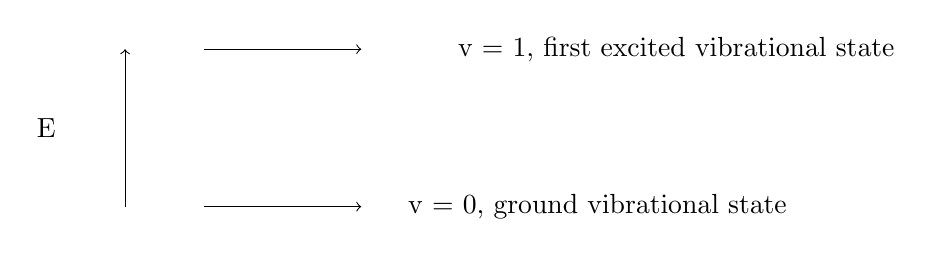
\begin{tikzpicture}
\draw[->] (0,0) --(0,2);
\draw [->] (1,0) -- (3,0);
\draw [->] (1,2) -- (3,2);
\node at (-1,1) {E};
\node at (7,2) {v = 1, first excited vibrational state};
\node at (6,0) {v = 0, ground vibrational state};
\end{tikzpicture}

What percentage of molecules are in the ground state? NOT 50\%!\newline
Depends on what? Temperature and energy separation between the two states E\newline
Given by the Boltzmann distribution\newline

So for molecules, the \underline{CRITICAL FACTORS} are determined by the quantised way in which energy is stored in the molecules
\end{frame}

\begin{frame}[allowframebreaks=0.6]
Consider a system composed of N particles\par
We can specify the total energy of the system, but we cannot be absolutely certain of how this energy is distributed -- and this applies despite the fact that we know the total energy \(E_{tot}\) is given by Eqn. 1:\par
\[E_{tot} = E_{translation} + E_{rotation} + E_{vibration} + E_{electronic}\]
Why can't we be certain? Because the energy is constantly being converted from one form to another by collision\par
The best we can do is to appreciate that we might be able to write down the average number of particles possessing a \underline{certain value} of energy which me can call \(\varepsilon\) but we must remember that each value of \(\varepsilon\) must be allowed an energy -- it cannot be just any energy!\par
So, we might conclude that of the total N particles, there are n\(_1\) particles having energy \(\varepsilon_1\), together with n\(_2\) particles having energy \(\varepsilon_2\) ... etc.\par
Assume that these distributions don't really change very much -- they stay constant. This then describes the \underline{statistical population} that we have to deal with.
\end{frame}

\begin{frame}[allowframebreaks]
So for now we have the following sets of particles (sets of populations)\newline
 
n\(_0\) particles with energy \(\varepsilon_0\)\newline
 
n\(_1\) particles with energy \(\varepsilon_1\)\newline
 
n\(_2\) particles with energy \(\varepsilon_2\)    etc\newline
 
This statement of \underline{populations} is known as the \underline{\textbf{configuration}} of the system\newline
Summary thus far:\newline
Have now defined the system, its \underline{populations} and its \underline{configuration}\newline
 
Adding some attempt at realism!\newline
Although the total energy cannot change, we can allow for instantaneous changes in the \underline{configuration}. 
The \underline{configuration} changes because the instantaneous populations change\newline

For example, we might, at one instant, have the following \underline{configuration}:\newline

\centering{n\(_0\) = N, n\(_1\) = 0, n\(_2\) = 0, n\(_3\) = 0, etc……  \newline \textbf{Can write this as \{N, 0, 0…\}}}\newline
 
Q. What would this mean? \newline
A. All particles are in the ground state for energy
\end{frame}

\begin{frame}[allowframebreaks]
But what about this one?    \quad   \{N-2, 2, 0, ….\} \medskip
 
Q. What would this mean? \newline
most of the particles ((N-2) of them in fact) are in the ground state, but 2 particles are in the 1st excited state.\newline

Statement: from a probability perspective this configuration is (much) more likely to occur than the configuration \{N, 0, 0…\}, particularly if N is large\newline
Why do we say this?\newline

\{N, 0, 0…\} can only be achieved in one way -- when none of the particles have any energy -- they are all in the ground state which we defined as having zero energy. 
 
But \{N-2, 2, 0, ….\} can be achieved in \(^1/_2\)(N-1) ways\newline
 
Why?
Starting with all N particles, choosing one particle to go into the higher state can be done N different ways\newline\smallskip
I can pick any particle -- so I have N choices
Once this has been done, to choose the second particle to put into the higher state I now have only (N-1) choices, because this is how many particles left in the lower state.\par\smallskip So the number of possible combinations here is N multiplied by (N-1), i.e. N(N-1) 
\end{frame}

\begin{frame}[allowframebreaks=0.7]
However, since I could start by picking particle number 34 say, then choose particle number 150, I would get EXACTLY the same \underline{configuration} if I picked particle number 150 first and particle number 34 second.\par\smallskip
 
Hence, to account for the fact that these are not distinguishable………..\par\smallskip
 
The number of choices becomes \textcolor{red}{\(^1/_2\)N(N-1)}\par\smallskip
 
Imagine what kind of number this would be?\newline\smallskip
If we took a mole of substance containing ca. \(6\times10^{23}\) particles:\newline
The chances of all particles being in the ground state is now represented by the probability of the \underline{configuration}
\{N, 0, 0…\} forming, and there was only 1 way that this could happen\par\smallskip
 
However, for the \underline{configuration} \{N-2, 2, 0, ….\}, with N = \(6\times10^{23}\) the number of choices becomes \(6\times10^{23}\times(6\times10^{23}- 1)\), which is a very, very large number!\par\smallskip
 
Given that there are this many chances available, it is obvious that if the system was left to equilibrate then it would ALWAYS be found in the second configuration.\par
 
\textcolor{red}{This is how basic probability theory is applied to the distribution of energy  between states}
\end{frame}

\begin{frame}[allowframebreaks=0.7]
\frametitle{The weight of the configuration}
A good analogy here is that if there is intelligent life on planet earth, and if there are an infinite number of planets in the universe, then it follows that statistically there must be intelligent life elsewhere in the universe. \textcolor{red}{What do you think about this?}\par\hrulefill\medskip


\textbf{The weight of the configuration, W}
 
Any general \underline{configuration} \{ n\(_0\), n\(_1\), n\(_2\), n\(_3\)…..etc\} can be achieved in W different ways.\par\smallskip
 
W is called the \underline{\textbf{weight}} of the \underline{configuration}.\par\smallskip
 
In general, W is given by eqn. 2\par\medskip
 
\begin{center} \(W = \frac{N!}{(n_0!\  n_1!\  n_2!\  n_3! …..)}\)    Eqn. 2\end{center}\par\medskip
 
Recall in mathematics, the \textbf{factorial} of a positive integer \textit{n}, denoted by \textit{n!}, is the product of all positive integers less than or equal to \textit{n}. For example\par\smallskip

\begin{center}5! = 5 × 4 × 3 × 2 × 1 = 120\end{center}
\end{frame}

\lecture{Interpreting the statistics}{Lecture 2}

\begin{frame}
\begin{columns}[onlytextwidth]
\begin{column}{.4\textwidth}
The weight of a configuration:\par
Interpretation is simple\par
The larger the weight, the more likely it will be for the configuration to arise	\par\medskip
So for N=2 in the table, the most likely configuration is \{1,1\}, because W=2 as compared to 1 for the other 2 possible configurations
\end{column}
\begin{column}{.6\textwidth}
\includegraphics[width=2.5in]{../graphics/weights}
\end{column}
\end{columns}
\end{frame}

\begin{frame}[allowframebreaks]
Eqn. 2 is a generalised version of the equation \(^1/_2\)N(N-1) and reduces to this for the specific case of the configuration 
\{N-2, 2, 0, ….\}\par\medskip
 
Can you see how this arises?\newline
Take a look at the denominator of eqn. 2:\par\medskip
 
How many particles are in the ground state?  n\(_0\) = N-2\par\smallskip
Hence,  n\(_0\)!  = (N-2) \(\times\) (N-3) \(\times\) (N-4) \(\times\) (N-5)….\par\medskip
 
How many particles are in the first excited state? n\(_1\) = 2\par\medskip
 
Hence n\(_2\)!  = 2\par\medskip
 
Putting this all together into eqn 2 we get \par\medskip
 
\[W = \frac{N\times(N-1)\times(N-2)\times(N-3)\times(N-4)….}{(N-2)\times(N-3)\times(N-4)\times(N-5)…. (2)}\]
\medskip
By cancellation we get \quad W = \(^1/_2\)N(N-1)
\end{frame}

\begin{frame}[allowframebreaks]
\frametitle{calculating weights}
We may encounter a mathematical conindrum:  

Consider Eqn. 2 again; what happens if any of the terms in the denominator are zero? As in the configuration \{N-2, 2, 0, ...\} for example  

Q. What is 0!?\newline
A. 0! = 1

\textbf{Proof:}\newline
If n! = 1x 2 x 3 x ... (n-2) x (n-1) x n  

Logically, n! can also be expresssed as n x (n-1)!  

Therefore, at n=1, using n! = n x (n-1)!  

1! = 1 x 0!

Which simplifies to 1 = 0!
\end{frame}


\begin{frame}<article:0>
\frametitle{Learning outcomes from today's lecture}
After studying this material you should be able to:
\begin{itemize}
\item Describe the configuration of a simple system of four molecules using the correct notation
\item Calculate the weight of different configurations of the simple system using Equation 2
\end{itemize}
\end{frame}


\begin{frame}
\frametitle{Summary thus far:}
 
We have now been through BASIC PROBILITY THEORY, which give the number of DISTINGUISHABLE ways that N objects can be placed in bins by putting n\(_i\) objects in bin number i etc.
 
\textcolor{red}{Next: to find the most likely configuration:}
 
We compared the two configurations \{N, 0, 0…\} and  \{N-2, 2, 0, ….\} and showed that when N was large (we took Avogadro's number) then the configuration where 2 particles were in the first excited state was much more likely to occur -- just on the basis of probability.

Now we ask the question: in a more general case, is there a \underline{configuration} that has such a large \underline{weight}, that it dominates over all others……..because if there is then it will determine the \textbf{properties} of the system

So, we need to find the values of n\(_i\), which lead to a maximum in W
\end{frame}

\begin{frame}[allowframebreaks=0.7]
\frametitle{Finding the configuration with the highest weight}
Not all configurations can be included in this analysis because they cannot both correspond to the same overall energy for the system
 
e.g. configuration \{N, 0, 0…\} corresponds to an overall energy of N\(\varepsilon_0\)
 
while configuration \{N-2, 2, 0, ….\} corresponds to an overall energy of (N-2)\(\varepsilon_0\) + 2\(\varepsilon_1\)
 
\medskip \textcolor{red}{\textit Since these are not the same they cannot be considered as both occurring at the same time.}
 
What this means is that when we look for the \underline{configuration} that has the greatest \underline{weight}, it MUST also match with the \underline{total energy criterion}, eqn. 3

\begin{center}
\fbox{\parbox{3in}{\(\sum_i n_i\varepsilon_i = E_{tot}\) \hspace{1in} Eqn. 3}}
\end{center}

Here the \(\sum\) symbol means sum up over all i  

\medskip We cannot arbitrarily vary all the possible populations, because there are only N particles in the system and this must \underline{NOT} change. This is said to be the \underline{total number criterion}, eqn. 4  
\begin{center}
\fbox{\(\sum_i n_i = N\)  \hspace{1in} Eqn. 4}
\end{center}  

Mathematically we can find the point where dW/dn = 0, the maximum in the graph of W vs n  

\medskip This will then point directly at the n values corresponding to the maximum in W

\medskip It turns out to be easiest to look at the criterion where not W itself, but \textbf{lnW} is a maximum.

\medskip lnW has a special status in statistical thermodynamics -- it is known as the \textbf{Configurational Entropy} (Next)
\end{frame}

\section{Statistical definition of entropy}

\begin{frame}[allowframebreaks=0.65]
\frametitle{The Statistical Meaning of Entropy -- the Configurational Entropy}
 
First consider the Thermodynamic Definition of Entropy:

The \textbf{first law of thermodynamics} is an expression of the principle of conservation of energy.

\medskip The law expresses that energy can be transformed, i.e. changed from one form to another, but cannot be created or destroyed.

\medskip It is usually formulated by stating that the change in the internal energy of a system is equal to the amount of heat supplied to the system, minus the amount of work performed by the system on its surroundings.


\medskip For a system undergoing only thermodynamic processes, i.e. a closed system that can exchange only heat and work, the change in the internal energy is given by:
\begin{center} \fbox{\textbf{\(dU = dq - dw\)}} \end{center}

where dU is the change in internal energy, dq is the change in the heat flow and dw is the change in work done. 


\medskip However, the concept of energy conservation alone does not account for the observation that natural processes have a \textbf{preferred direction} of progress. 

 
\medskip For example, the \textbf{2\(^{nd}\) Law} of thermodynamics states that spontaneously, heat always flows to regions of lower temperature \textcolor{red}{(increasing randomness)}, never to regions of higher temperature without external work being performed on the system.  

 
\medskip Yet the 1st law is completely symmetrical with respect to the initial and final states of an evolving system?


\medskip The key concept for the resolution of the issue introduced by the second law of thermodynamics is the definition of a new property, \textcolor{red}{\textbf{the entropy}}.


\medskip How does this quantity evolve?
If the only work done by or on the system is expansion work, then  \(-dw = -PdV\)


\medskip Now we know that the enthalpy is obtained from the sum of the internal energy and the work done overall

\begin{center}
 H = U +PV …. and hence that dH = dU+ PdV at constant P 
\end{center}
(because the term VdP disappears from the differential)

\medskip Substituting for dU = dq –PdV we get\newline
\medskip \(dH = dq - PdV+ PdV\), or more simply that \(\Delta H = dq\)\newline
\medskip Given that \(\Delta G = \Delta H - T\Delta S\) and at equilibrium \(\Delta G=0\) \newline
\medskip Then \(0 =  \Delta H - T\Delta S  =  dq- T\Delta S\) and hence, \(\Delta S = dq/T\)

\medskip An entropy (S) change is the infinitesimal variation of the internal energy of a system driven by the transfer of heat (q), divided by the equilibrium temperature (T) of the system: dS = dq/T

\bigskip Statement of the 2nd Law:

\textcolor{red}{\textbf{The entropy of an isolated system that is in thermal equilibrium is constant and has reached its maximum value} (because spontaneously entropy can only increase or in a special case, stay the same, never decrease)}
 
\medskip So we define equilibrium as the point of maximum entropy.

\medskip But how does this relate to the statistical approach?
\end{frame}

\begin{frame}[allowframebreaks]
\frametitle{Entropy and Configuration}
When the temperature is raised the entropy of any system tends to increase for two reasons;  
\begin{itemize}
\item the increasing thermal motion of the molecules tends to make the assembly occupy a volume greater than that required to pack the molecules together in the (perfect, crystalline)  solid state

\item an increase in temperature leads to the promotion of molecules from the ground state or low-lying energy states to higher levels.  The extent to which this occurs is described by the appropriate distribution, e.g the \textbf{Boltzmann distribution} (next)
 \end{itemize}
 
We should therefore expect a definite relation to exist between entropy, thought of as the \textbf{‘randomness’} of a system, and the \textbf{probability} or number of different ways (\textbf{weight})  W,  in which a system with a given number of particles and of constant energy can be realized.
 
\medskip The greater the probability, the more likely the configuration will correspond to the true equilibrium configuration
This means the point of maximum entropy. So, \textcolor{red}{\textbf{\textsl{the greater the probability, the greater the entropy.}}}
\end{frame}

\section{Boltzmann distribution}

\begin{frame}[allowframebreaks]
\frametitle{Boltzmann}
How does this work? \quad Consider the entropies of two independent parts of an assembly, parts 1 and 2
 
\smallskip These entropy terms may be added to give the entropy of the whole system, e.g.:
 
\begin{center} \textcolor{red}{\(S_{tot} = S_1 + S_2\)} \end{center}
 
On the other hand if the number of ways of distributing particles in one part, (the weight) is W\(_1\), and the number of ways of distributing particles in the other part is W\(_2\)
 
Then the number of ways of distributing the whole system, (the probability) is the product:
\begin{center} \textcolor{red}{Probability \(= W_1 \times W_2\)} \end{center}
Thus we have different behaviour for entropy -- additive and the weights of the configuration -- multiplicative.


This strongly suggests a relation of the type:
\begin{center} \textcolor{red}{\(S \propto lnW \)} \end{center}

With the proportionality constant k, so that \(S = klnW\)

Why? Because this would be consistent with the following argument:\smallskip

\fbox{\parbox{4in}{\(S_{tot} = klnW = kln(W_1\cdot W_2) = klnW_1 + klnW_2 = S_1 + S_2\)\medskip

So, by inspection: \(S_1 = klnW_1\) and \(S_2 = klnW_2\)\medskip

or generally, \(S=klnW\)}}\smallskip

So because when log terms are added the result is to multiply the numbers together, this approach is consistent.

The equation is called the Boltzmann equation, while k is the Boltzmann constant.

This equation appears on Boltzmann's grave!
\begin{figure}
\includegraphics[height=1.5in]{../graphics/Boltzmann}
\end{figure}

\end{frame}

\textcolor{red}{So for the most perfectly arranged crystal, at any real temperature, i.e. not at absolute zero (which cannot be achieved anyway for the same reason), there must be some \underline{entropy}, for example in the form of \underline{vacancies}, like Schottky or Frenkel defects (CM3025). \textbf{3\(^{rd}\) law of thermodynamics}}


\begin{frame}
\frametitle{class exercise}
Example of the application of the statistical approach

Summer Examination 2015:

A system contains 4 equivalent molecules (N=4). The molecules are distributed over a series of 4 energy levels labelled 1, 2, 3 and 4, having energies equal to \( 0, \varepsilon, 2\varepsilon\) and \(3\varepsilon\) respectively. Given that the total energy of the system is \(8\varepsilon\), determine the 3 possible allowed configurations as described by the sets of possible populations written as \(\{n_0, n_1, n_2, n_3\}\) where the n values represent the populations of the levels in question. Remember that any allowed configuration must satisfy both the ‘total number’ and ‘total energy’  criteria.

Determine the weight W for each configuration and hence identify the most likely configuration.  Calculate the entropy  S associated with this configuration.	
\end{frame}

\begin{frame}<article:0>
\frametitle{Learning outcomes from today's lecture}
After studying this material you should be able to:
\begin{itemize}
\item Find the configuration of a system with the highest weight = find the most probable configuration
\item Use the \underline{total energy crietrion} and \underline{the total number criterion}
\item explain the statistical meaning of entropy
\end{itemize}
\end{frame}

\lecture{The Boltzmann Distribution}{Lecture 3}

\begin{frame}[allowframebreaks]
\frametitle{The Boltzmann distribution from a statistical thermodynamics perspective}
Recall: to find the maximum possible Weight, need to set dW/d\(n_i\) = zero and find which \(n_i\) values allow for this to occur\smallskip

As suggested previously (Lecture 2) , it turns out to be easiest to look at the criterion where not W itself, but lnW is a maximum, so we use the \textbf{configurational entropy}\smallskip

When a \underline{configuration} n\(_i\) changes slightly, we write the \underline{altered configuration} as \(n_i + dn_i\)\smallskip
 
This then changes the lnW term slightly, which we then express as 
\begin{center}
\(dlnW  = \sum_i \left( \frac{\delta lnW}{\delta n_i}\right)  dn_i\) \hspace{1in} \fbox{\parbox{1in}{\tiny Note: the \(\delta\) is known as a partial derivative and is used when one needs to differentiate with respect to one term, in this case n\(_i\) , keeping all other terms constant.
}}
\end{center}

This complicated looking equation simply states that the small change in \underline{weighting} is induced by a change in \underline{configuration}
\end{frame}

\begin{frame}[allowframebreaks]
\frametitle{Solving for n\(_i\) when dlnW = 0}
So, at the maximum of the curve the term dlnW  = 0.

But: we can't just see what this does to the n\(_i\) term without considering that the n\(_i\) are NOT independent. 
 
Why are they not independent?
 
Because of our two criteria introduced earlier :

\medskip
\(\sum_i \varepsilon_i  dn_i  =    0            	\)\newline\smallskip
and\newline\smallskip
\(\sum_i dn_i  =    0            	\)\newline

\textit{\textcolor{red}{These are going to be called our two formal constraints}}
 
This is a tough problem to solve, but there are ways of doing this mathematically. 
 
One solution makes use of an approach called the \textit{Method of Undetermined Multipliers}, invented by the mathematician Lagrange.
\end{frame}

\begin{frame}
\frametitle{Using Lagrange's method to incorporate our formal constraints}
This says: \textit{our two formal constraints must be added to our equation for d(lnW), in a way that allows us to vary how much they contribute to the answer. }\par\medskip
 
This is done by just putting these two constraints into the equation above, ……..but multiplying each of them by a constant, which we don't have to evaluate until the solution is basically found (!)\par\medskip
 Hence the name \textbf{'undetermined multiplier‘}\par

What does this then give us? If we choose to multiply by the constants
\(-\beta\) and \(\alpha\) (........and a certain amount of hindsight has been used here!)\par\medskip
 
\(dlnW  = \sum_i \left( \frac{\delta lnW}{\delta n_i}\right) dn_i +  \textcolor{red}{\alpha \sum_i dn_i  -  \beta \sum_i \varepsilon_i  dn_i}\)           

where the constraints multiplied by their constants are highlighted in red
\end{frame}

\begin{frame}[allowframebreaks]
This can be simplified to:\par\bigskip
 
\[d(lnW)  = \sum_i \left\{\left(\frac{\delta lnW}{\delta n_i}\right)   +  \alpha  -  \beta \varepsilon_i \right\} dn_i \]
  
Now the use of this method means that all the n\(_i\) terms can genuinely be thought of as independent of each other, because we can naturally avoid those values which cannot exist for the system.\par\bigskip

When we are at the condition defining the maximum in lnW, namely that:\par

dlnW  =  0, then
\begin{center}
\fbox{\(\sum_i \left\{\left(\frac{\delta lnW}{dn_i}\right)   +  \alpha  -  \beta \varepsilon_i \right\} dn_i     =  0\)}
\end{center}
When this result applies, the n\(_i\) values MUST have their most probable values, and we can write these as n\(_i^*\)
\end{frame}

\begin{frame}[allowframebreaks=0.7]
In order to solve this equation we have to somehow evaluate the term 
\( \frac{dlnW}{dn_i}\)\par\medskip
 
There is a way of simplifying this, called Stirling's approximation, which states that :\par\medskip
 
\[lnx! = xlnx - x\]\par\medskip
 
Writing out lnW in full we get:\par\medskip
 
\[lnW   = ln\left\{\frac{N!}{(n_0!  n_1!  n_2!  n_3! …..)} \right\} \]  (just from our previous definition of W)

This may be written as:

\[lnW   = lnN! - ln(n_0!  n_1!  n_2!  n_3! …..) = NlnN - \sum_i ln\ n_i\] 
 
Now using Stirling's approximation we can write:
 
\[lnN! = NlnN - N\]
\end{frame}

\begin{frame}[allowframebreaks]
Also given that:\par\medskip
 
\(ln(n_0!  n_1!  n_2!  n_3! …..)      = \sum_i ln (n_i!)\) \hspace{1cm}        we can \textit{also} write that:\par
 
\[ln(n_0!  n_1!  n_2!  n_3! …..)      = \sum_i n_i ln(n_i)  - n_i   \]

So this result arises because we have applied Stirling's approximation to both the N and n\(_i\) terms\par\medskip
 
Putting these two 'adjusted’ terms together we get:\par\medskip

\(lnW = NlnN \textcolor{red}{- N}    - \sum_i n_i ln(n_i)  \textcolor{red}{- n_i}\)     \hspace{1cm} or\par\medskip
 
\(lnW = NlnN - \sum_i n_i ln(n_i)\) \hspace{0.5cm}  …where did the terms in red go?\par\medskip

We may assume that since N is going to be very large, then NlnN is going to be extremely large and so we can NEGLECT the \textcolor{red}{N} term and a similar argument applies for  the \textcolor{red}{\(-n_i\)}  term. 
\end{frame}

\begin{frame}[allowframebreaks]
Recall what we are after? We want to know \(\frac{\delta lnW}{\delta n_i}\)\par\medskip
 
Since N is a constant, and hence lnN is also a constant, then the partial derivative of the  term NlnN with respect to \(n_i\) must be eual to zero\par
\textcolor{red}{(In other words the total number of particles in the system cannot change)}\par\medskip
 
What else is constant?\par
Q. What does the term \(\sum_i n_i \) equal?\par
A. N, which is a constant.\par\medskip

Thus we find that \(\frac{\delta lnW}{\delta n_i}\) reduces as follows:\par\medskip

From the above, \(lnW = NlnN - \sum_i n_i ln(n_i)\)\par\medskip 
Now try to differentiate:\par\medskip

\begin{align*} \frac{\delta lnW}{dn_i} &= \textcolor{red}{NlnN} – \sum_i n_i \frac{\delta ln(n_i)}{\delta n_i}\\
\frac{dlnW}{dn_i} &= \frac{dN}{dn_i}lnN + N \frac{dlnN}{dn_i} - \sum_i \frac{d(n_iln\ n_i)}{dn_i}\\
&= lnN + N\frac{1}{N} - (ln\ n_i +1)\\
&= lnN + 1 - ln\ n_i - 1\\
&= lnN - ln\ n_i = -(ln\ n_i - lnN)\\
\end{align*}
 
which then reduces to \(\frac{\delta lnW}{\delta n_i}  =  - ln\left(\frac{n_i}{N}\right)\)\par   \medskip

\begin{flushright}\fbox{\parbox{1in}{\tiny Maths help:\newline
Remember that \(\frac{dlnx}{dx} = \frac{1}{x}\)\newline so, \(\frac{\delta ln(n_i)}{\delta n_i} = \frac{1}{n_i}\)\newline Then differentiate by parts:\newline \(\frac{\delta}{\delta n_i} \left\{n_i ln(n_i)\right\} = \frac{n_i}{n_i } + 1\cdot ln(n_i) = 1 + ln(n_i)\)\newline
But \textbf{when \(n_i\) is large}, this reduces to just \(ln(n_i)\)}}\par\medskip
\end{flushright}

Where did the summation go?  Since all the \(n_i\) terms must be independent, then the only term that does not disappear is the term \(\frac{\delta n_i}{\delta n_i}  = 1\)\par\medskip

so finally, \(\left(\frac{\delta lnW}{\delta n_i}\right) + \alpha - \beta \varepsilon_i = 0\) becomes\par
\[-ln\left(\frac{n_i^*}{N}\right) + \alpha - \beta \varepsilon_i = 0\]

and now the \(n_i\) terms must be written as \(n_i^*\) to signify that this represents the most probable populations\par\medskip

Solving this equation for \(n_i^*\) yields the following result:\par\medskip
\[\frac{n_i^*}{N} = e^{[\alpha - \beta \varepsilon_i]} = e^\alpha e^{-\beta\varepsilon_i}\]
or
\[n^*_i = N e^\alpha e^{-\beta\varepsilon_i}\]

So what is this?\par
This is the most \underline{probable population} of the state with energy \(\varepsilon_i\)\par
... \textit{which now begins to look like a Boltzmann distribution ...}\par\medskip
Now we just have to figure out what \(\alpha\) and \(\beta\) are\par\medskip

Now we know that we can write:\par\medskip

\(N=\sum_i n_i^*\) and so we can also write \(N=Ne^{\alpha}\sum_i \cdot e^{-\beta \varepsilon_i}\)\par\medskip

If this is the case we may also write: \(1 = e^{\alpha}\sum_i \cdot e^{-\beta \varepsilon_i}\) so:\par\medskip

\[e^\alpha = \frac{1}{\sum_i e^{-\beta \varepsilon_i}} = \frac{n_i^*}{Ne^{-\beta\varepsilon_i}}\]\par\medskip

Substituting for \(e^\alpha\) yields:\par
\begin{center}
\setlength{\fboxrule}{5pt}
\fbox{\parbox{2.5in}{\[n_i^* = \frac{Ne^{-\beta \varepsilon_i}}{\sum_i e^{-\beta \varepsilon_i}}\]\newline This is the Boltzmann distribution}}
\end{center}
\end{frame}

\begin{frame}{The partition function}
\only<1>{
The denominator in the equation is referred to as the \textbf{partition function}, \textit{q}, and is defined as:

\[ q = \sum_i e^{-\beta \varepsilon_i}\]

The partition function represents the sum over all terms that describes the probability associated with the variable of interest, in this case \(\varepsilon_i\), or the energy of level \textit{n}. 
}
\only<2>{
Using the partition function with the above, the probability of occupying a given energy level,\(p_i\) becomes

\[p_i = \frac{n_i}{N} = e^\alpha e^{-\beta \varepsilon_i} = \frac{e^{-\beta \varepsilon_i}}{q}\]

\begin{alertblock}{The final result}
the last equation is the result of interest. It quantitatively describes the probability of occupying a given energy for the dominant configuration of energy. It is the \textbf{Boltzmannn distribution}.

The Boltzmann distribution is a statement of probability and the partition function serves to \textit{normalise} the probability distribution.
\end{alertblock}
}
\end{frame}

Another way of stating it is that the quantized energy levels of the molecular (or atomic) system are embedded in the \textbf{molecular partition function}.

\subsection{Physical meaning of the Boltzmann distribution}

\begin{frame}{The physical meaning of the Boltzmann distribution}
\only<1>{Remember the central postulate of statistical mechanics: \begin{quote} Every possible microstate of an isolated assembly of units occurs with equal probability \end{quote}

This cannot be verified experimentally. But what does it mean, anyway?

\bigskip We will accept the following features:
}
\only<2>{
\begin{itemize}
\item[1] All microstates are equally probable; however one has the greatest probability of observing a microstate associated with the dominant configuration
\item[2] Configurations having a significant number of microstates will be only infinitesimally different from the dominant configuration. The macroscopic properties of the system will be identical to that of the dominant configuration. Therefore, with overwhelming probability one will observe a macroscopic state of the system characterised by the dominant configuration
\end{itemize}
}
\only<3>{
\begin{itemize}
\item[3] Continued monitoring of a system will result in the observation of macroscopic properties of the system that appear unchanging, although energy is still being exchanged between the units of our assembly. This macroscopic state of the system is called the \textbf{equilibrium state}
\item[4] given items 1 through 3, the equilibrium state of the system is characterised by the dominant configuration
\end{itemize}
}
\only<4>{
\begin{alertblock}{Implication}
The Boltzmann distribution law describes the energy distribution associated with a chemical system at equilibrium
\end{alertblock}

\bigskip {\large \textbf{The fact that all microstates have equal probability of being observed does not translate into an equal probability of observing all configurations!}}
}
\end{frame}

\subsection{The definition of \(\beta\)}
\begin{frame}{The definition of \(\beta\)}
\only<1>{
To use the Boltzmann distribution we need a definition for \(\beta\) that involves measureable system parameters.

\medskip We'll derive one by considering the variation in weight, \textit{W} as a function of total energy contained by an assembly of units, \textit{E}.

\medskip Imagine an assembly of 10 oscillators having only three quanta of total energy. The majority of oscillators will occupy the lowest energy states and the weight corresponding to the dominant configuration should be small. As energy is deposited ito the system, the oscillators will occupy higher energy states and the denominator in the equation \(W = \frac{N!}{n_0!n_1!n_2!...n_i!} = \frac{N!}{\prod_i n_i!}\) will be reduced, thereby increasing \textit{W}. 

\smallskip So we expect \textit{W} and \textit{E} to be correlated.
}
\only<2>{
\medskip We determine the relationship between \textit{W} and \textit{E} by taking the natural log of the last equation:

\[lnW = lnN! - ln\prod_i n_i! = lnN! - \sum_i ln\ n_i!\]

We are interested in the change in \textit{W} with respect to \textit{E}, so we have to differentiate \textit{W}:

\begin{align*}
dlnW &= -\sum_i d\ ln\ n_i!\\
&= -\sum_i ln\ n_idn_i
\end{align*}

The last results used Stirling's approximation to evaluate \(ln\ n_i!\) and recognising that \(\sum_i dn_i = 0\).
}
\only<3>{
Now we use the Boltzmann relationship to define the ratio between the occupation number for an arbitrary energy level, \(\varepsilon_i\) versus the lowest, or ground energy level (\(\varepsilon_0 = 0\)):

\[\frac{n_i}{n_0} = \frac{\frac{Ne^{-\beta\varepsilon_i}}{q}}{\frac{Ne^{-\beta\varepsilon_0}}{q}} = e^{-\beta\varepsilon_i}\]
\[ln\ n_i = ln\ n_0 - \beta\varepsilon_i\]

\smallskip Putting this back into the expression for \(dlnW\) gives:

\begin{align*}
dlnW &= -\sum_i (ln\ n_0 - \beta\varepsilon_i)dn_i\\
&= -ln\ n_0\sum_i dn_i + \beta\sum_i \varepsilon_idn_i
\end{align*}
}
\only<4>{
\smallskip The first summation represents the total change in occupation number and it is equal to the change in the total number of oscillators in the system. But the system is closed with respet to the number of oscillators, \(dN = 0\) so the summation is equal to zero.

The second sum represents the change in total energy of the system (\textit{dE}) accompanying the deposition of energy into the system: \(\sum_i \varepsilon_idn_i = dE\).

With the last equality, the relationship between \(\beta\), weight and total energy is derived:

\begin{center}\fbox{\parbox{1in}{ \[ dlnW = \beta dE\]}}\end{center}
}
\only<5>{
\smallskip The boxed equality provides insight into the physical meaning of \(\beta\). We recognised initially that the weight increases in proportion with the energy available to the system; \(\beta\) is simply the proportionality constant in that relationship.

\textrightarrow \smallskip \(\beta\) must have units of inverse energy.

\smallskip Thermodynamics dictates that because temperature is a measure of internal kinetic energy, an increase in the energy will be accompanied by an increase in the temperature of an assembly.

\smallskip \(\beta\) must be inversely related to \textit{T}. Unit analysis of the last equality in the framed box we also know that \(\beta\) must have units of inverse energy. We include a proportionality constant in the relationship between \(\beta\) and \textit{T}.
}
\only<6>{
The final expression for \(\beta\):
\begin{center}\fbox{\parbox{1in}{ \[\beta = \frac{1}{kT}\]}}\end{center}

The constant, \textit{k} is \textbf{Boltzmann's constant} and has has the value \(1.381\times10^{-23}\) JK\(^{-1}\).

The product of \textit{k} and Avogadro's number is equal to \textit{R}, the ideal gas constant (8.314 J mol\(^{-1}\) K\(^{-1}\).
}
\end{frame}

\begin{frame}<article:0>
\frametitle{Learning outcomes from today's lecture}
After studying this material you should be able to:
\begin{itemize}
\item write (not derive) the equation for the Boltzmann distribution
\item apply Stirling's approximation for lnN!
\item explain the physical meaning of the Boltzmann distribution
\item use the partition function to perform calculations
\end{itemize}
\end{frame}

\lecture{Ensembles, partition functions and energy}{Lecture 4}

\section{The ensembles}

\begin{frame}{What are ensembles?}
\only<1>{
A central concept in statistical thermodynamics is the relationship between the microscopic descritption of individual molecules and the macroscopic properties of a collection of molecules.

\medskip An \textbf{ensemble} is defined as a collection of identical units or replicas of a system. For example, a mole of water can be envisioned as an ensemble with Avogadro's number of identical units of water molecules. The ensemble provides a theoretical concept by which the microscopic properties of matter can be related to the corresponding thermodynamic system properties.

\medskip \fbox{\parbox{.9\textwidth}{The average value for a property of the ensemble corresponds to the timeaveraged value for the corresponding macroscopic property of the system}}
}

\only<2>{
\medskip So for individual units in the ensemble, let's say we measure the energy content of each unit at a single time and the measured unit energies are used to determine the average energy for the ensemble.

\medskip According to the postulate above, this energy will be equivalent to the average energy of the ensemble measured over time. This idea was first formulated by J. W. Gibbs in the late 1880s. It lies at the heart of statistical thermodynamics.

\medskip We classify ensembles according to how their members interact with outside systems.
}
\end{frame}
\begin{frame}{ensembles and interaction with the surroundings}
\only<1>{
If there is no interaction at all, it is called a ``\textbf{microcanonical ensemble}''.

\smallskip In a ``\textbf{canonical ensemble}'' the members interact \textit{thermally and/or mechanically} with an outside system. An example is the oxygen molecules in our atmosphere. The probability for any molecule to be in a certain quantum state is reflected in the fraction of all oxygen molecules that are in that state. Because each molecule interacts thermally and mechanically, but not diffusively (N = one molecule for each member) with the atmosphere, altogether they form a canonical ensemble.
}
\only<2>{
\smallskip In addition to possible thermal and mechanical interaction, the members of a ``\textbf{grand canonical ensemble}'' interact diffusively with their environment. An example would be the large number of identical quantum states, each of which has particles entering and leaving it. Another example would be a large number of identical ice crystals interacting diffusively with the moisture in the air.
}
\end{frame}
\subsection{The microcanonical ensemble}
\subsection{The canonical ensemble}
\begin{frame}{The canonical ensemble}
\only<1>{
To connect ensemble average values and thermodynamic properties, we begin by imagining a collection of identical copies of the system.

\smallskip These copies are held fixed in space such that they are distinguishable.

\smallskip The volume, V, temperature, T, and number of particles in each system, N, are constant. An ensemble in which \textbf{V, T and N are constant} is referred to as a \textbf{canonical ensemble}.
}
\only<2>{
In this canonical ensemble, each member is held in a temperature bath so that the total ensemble energy is constant. The walls that define the the volume of the units can conduct heat, allowing energy exchange with the surroundings. We will develop a statistical description of this ensemble.
}
\only<3>{
\begin{figure}[h]
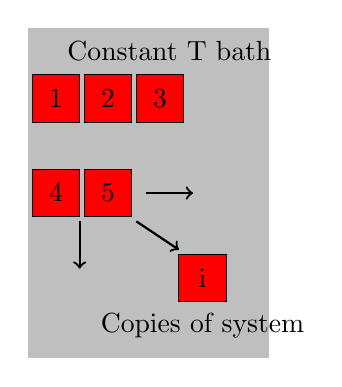
\begin{tikzpicture}[scale=0.6]
\path [fill=lightgray] (0,-1) rectangle (5.1,6);
%\draw[help lines] (0,0) grid (6,6);
\draw[fill=red] (.1,4) rectangle (1.1,5); \node at (.6,4.5){1};
\draw[fill=red] (1.2,4) rectangle (2.2,5); \node at (1.7,4.5){2};
\draw[fill=red] (2.3,4) rectangle (3.3,5); \node at (2.8,4.5){3};
\draw[fill=red] (.1,2) rectangle (1.1,3); \node at (.6,2.5){4};
\draw[fill=red] (1.2,2) rectangle (2.2,3); \node at (1.7,2.5){5};
\draw[->,thick] (2.3,1.9) -- (3.2,1.3);
\draw[->,thick] (2.5,2.5) -- (3.5,2.5);
\draw[->,thick] (1.1,1.9) -- (1.1,0.9);
\node at (3,5.5){Constant T bath};
\draw[fill=red] (3.2,1.2) rectangle (4.2,.2); \node at (3.7,.7){i}; \node at (3.7,-.3){Copies of system};
\end{tikzpicture}
\caption{The canconical ensemble is comprised of a collection of identical systems having fixed temperature, volume and number of particles. The arrows indicate that an infinite number of copies of the system comprises the ensemble}
\end{figure}
}	
\only<4>{
The total energy of the ensemble can be expressed as 
\[ E_c = \sum_i n_iE_i\]

The terms \(n_i\) are the occupation numbers corresponding to the number of ensemble members having energy \(E_i\). 

The weight, \(W_c\), associated with a specific configuration of energy among the \(N_c\) members of the ensemble is given by
\[W_c = \frac{N_c!}{\prod_i n_i}\]

This relationship can be used to derive the probability of finding an ensemble unit at energy \(E_i\):

\begin{equation}\label{ensembleprob}
p(E_i) = \frac{W_ie^{-\beta E_i}}{Q}
\end{equation}
}
\only<5>{
This equation looks similar to the probability expression. \(W_i\) can be thought of as the umber of states present at a given energy \(E_i\). 

\medskip The quantity \(Q\) in the equation is the \textbf{canonical partition function} and is defined as:

\begin{equation}\label{canpart}
 Q = \sum_i e^{-\beta E_i}
\end{equation}
}
\only<6>{
In the equation the summation is over all energy levels.

\medskip The probability depends on two things: \(W_i\), or the number of states present at a given energy (which increases with energy) and a Boltzmann term \(e^{-\beta E_i} / Q\) that describes the \textbf{probability of an ensemble unit having energy \(E_i\)} (which decreases exponentially with energy).

\medskip The product of these terms will reach a maximum corresponding to the average ensemble energy.
}
\only<7>{
\begin{figure}[h] \label{prod}
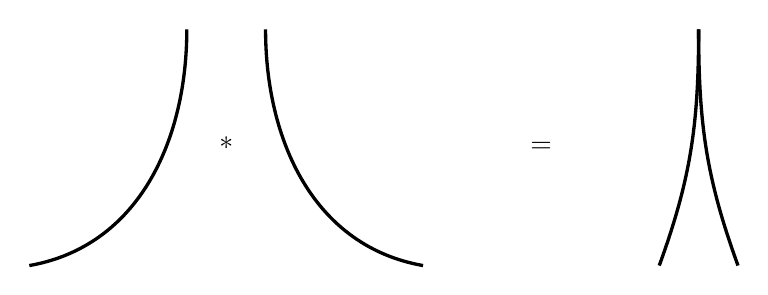
\begin{tikzpicture}
\draw[very thick] (0,0) to [out=10,in=270] (2,3); \node at (2.5,1.5){*}; \draw[very thick] (3,3) to [out=270,in=170] (5,0);
\node at (6.5,1.5){=}; \draw[very thick] (8,0) to [out=70,in=270] (8.5,3); \draw[very thick] (8.5,3) to [out=270,in=110] (9,0);
\end{tikzpicture}
\caption{Product of an increasing and a decreasing function produces a narrow band of non-negligible values}
\end{figure}
}
\only<8>{
\begin{alertblock}{Result}
An individual unit of the ensemble will have an energy that is equal to or extremely close to the average energy, and units having energy far from this value will be exceedingly rare
\end{alertblock}

\begin{exampleblock}{Example: swimming pool}
If the thermometer at one side of the pool shows 18\(^\circ\)C, we don't expect a liter of water at the other end of the pool will freeze. \\ The temperature at one end of the pool is enough to characterise the temperature of the water in any part of the pool.
\end{exampleblock}
}
\end{frame}

\lecture{Entropy and thermodynamic functions}{Lecture 5}

\subsection{The grand canonical ensemble}

\section{The ensemble partition function}
\begin{frame}{More about the ensemble partition function}
\only<1>{
The partition function is a tool that is used to simplify many calculations.

\medskip When a small system is interacting with a large reservoir, the probability for it to be in state \textit{s} is \(P_s = CE^{-\beta E_s}\), and the mean value of any property \textit{f} of the small system is given by
\begin{equation}
\overline{f} = \sum_s f_sP_s
\end{equation}
with \(P_s = Ce^{-\beta E_s}\)

\smallskip The problem is that the sum over states can include a very large number of terms and the calculation must be repeated for every property \textit{f} that we want to study.
}
\only<2>{
The partition function facilitates these otherwise tedious calculations. Once the sum is done and the partition function is known, many different properties can be calculated directly from it.
\bigskip

\subsection{Q and q for an ideal gas}
The canonical partition function, \textit{Q}, (for the whole ensemble) is related to the partition function describing each member of the ensemble, \textit{q}.

\smallskip We will only discuss systems consisting of independent ``ideal'' particles with negligible interactions between particles.
}
\only<3>{
The relationship between \textit{Q} and \textit{q} starts by considering an ensemble made up of two distinguishable units, A and B.

For this simple ensemble, the partition function is

\[ Q = \sum_i e^{-\beta E_i} = \sum_i e^{-\beta (\varepsilon_{A_i} + \varepsilon_{B_i})}\]

The terms \(\varepsilon_{A_i}\) and  \(\varepsilon_{B_i}\) refer to the energy levels associated with unit A and B

Assuming the energy levels are quantized such that they can be indexed as 0, 1, 2, etc., the equation becomes:
}
\only<4>{
\begin{align*}
Q &= \sum_i e^{-\beta (\varepsilon_A + \varepsilon_B)} =  e^{-\beta (\varepsilon_{A_0} + \varepsilon_{B_0})} + e^{-\beta (\varepsilon_{A_0} + \varepsilon_{B_1})} + e^{-\beta (\varepsilon_{A_0} + \varepsilon_B{_2})} + ...\\
& + e^{-\beta (\varepsilon_{A_1} + \varepsilon_{B_0})} + e^{-\beta (\varepsilon_{A_1} + \varepsilon_{B_1})} + e^{-\beta (\varepsilon_{A_1} + \varepsilon_B{_2})} +...\\
& + e^{-\beta (\varepsilon_{A_2} + \varepsilon_{B_0})} + e^{-\beta (\varepsilon_{A_2} + \varepsilon_{B_1})} + e^{-\beta (\varepsilon_{A_2} + \varepsilon_B{_2})} + ...\\
& = (e^{-\beta \varepsilon_{A_0}} + e^{-\beta \varepsilon_{A_1}} + e^{-\beta \varepsilon_{A_2}} + ...)(e^{-\beta \varepsilon_{B_0}} + e^{-\beta \varepsilon_{B_1}} + e^{-\beta \varepsilon_{B_2}} + ...)\\
& = (q_A)(q_B)\\
& = q^2
\end{align*}
}
\only<5>{
The ensemble units are identical so the partition functions are also identical.

\fbox{\parbox{.9\textwidth}{For a system with N \textbf{distinguishable units}, the canonical partition function is simply the product of unit partition functions:
\begin{center} \(Q = q^N\) \quad for \textit{N} distinguishable units \end{center}}}

\medskip The system can be any size, including just a single molecule. The quantized nergy levels of a molecyular (or atomic) system are embedded in the \textbf{molecular partition function}, \textit{q} and this partition function can be used to define the partition function for the ensemble, \textit{Q} and \textit{Q} can be related to the thermodynamic properties of the ensemble.
}
\only<6>{
\medskip But what if the units are indistinguishable? For example for a system in the gaseous state.

For a system of \textit{N} indistinguishable particles  the total number of permutations is divided by \textit{N}!
\begin{center}
\fbox{\parbox{.5\textwidth}{The canonical partition function:\\
 \(Q = \frac{q^N}{N!}\) \quad for \textit{N} indistinguishable units }}
\end{center}
}
\end{frame}
\subsection{Energy and the canonical partition function}
\begin{frame}{Calculating energy using the partition function}
\only<1>{
Let's consider the \textbf{average energy} content of an ensemble unit, \(\langle\varepsilon \rangle\). This is simply the \textbf{total energy} of the ensemble, \textit{E}, divided by the number of units in the ensemble, \textit{N}:
\[\langle \varepsilon \rangle = \frac{E}{N} = \frac{\sum_i\varepsilon_in_i}{N} = \sum_i\varepsilon_i\frac{n_i}{N}\]


In this equation, \(\varepsilon_i\) is the level energy and \(n_i\) is the occupation number for ith elevel.

The ensemble is partitioned so that there is one atom or molecule in each unit. The Boltzmann distribution for a series of nondegenerate energy levels is
\[\frac{n_i}{N} = \frac{e^{-\beta\varepsilon_i}}{q}\]
}
\only<2>{
In the expression above, \textit{q} is the molecular partition function. Substituting the second expression into the first one gives:
\[\langle\varepsilon\rangle = \sum_i\varepsilon_i\frac{n_i}{N} = \frac{1}{q}\sum_i\varepsilon_ie^{-\beta\varepsilon_i}\]

Consider the derivative of the molecular partition function with respect to \(\beta\), which is given by
\[\frac{-dq}{d\beta} = \frac{d}{d\beta}\left(\sum_i\varepsilon_ie^{-\beta\varepsilon_i}\right)\]

Rewrite the expressions above to obtain the following expressions for the average unit energy and total ensemble energy:
}
\only<3>{
\begin{center}
\fbox{\parbox{.6\textwidth}{
\[\langle\varepsilon\rangle = \frac{-1}{q}\left(\frac{dq}{d\beta}\right) = -\left(\frac{d\ lnq}{d\beta}\right)\]
\medskip
\[E = N\langle\varepsilon\rangle = \frac{-N}{q}\left(\frac{dq}{d\beta}\right) = -N\left(\frac{d\ lnq}{d\beta}\right)\]
}}
\end{center}

The expressions in the box above are sometimes easier to evaluate by taking derivative with respect to \textit{T} rather than \(\beta\).
\begin{center} \fbox{\textbf{definition:} \( \beta = (kT)^{-1}\)} \end{center}

\[\frac{d\beta}{dT} = \frac{d}{dT}(kT)^{-1} = -k(kT)^{-2} = -\frac{1}{kT^2}\]
}
\only<4>{
Using the last expression, the average and total energy can be written as follows:
\begin{center}
\fbox{\parbox{.6\textwidth}{
\[\langle\varepsilon\rangle = kT^2\left(\frac{d\ lnq}{dT}\right)\]
\medskip
\begin{equation}\label{NkT}
E = NkT^2\left(\frac{d\ lnq}{dT}\right)
\end{equation}
}}
\end{center}

This means that \textit{E} will change with temperature, as we are used to from thermodynamics. The next example involves an ensemble comprised of particles with two energy levels, so it can be referred to as a \textbf{two-level system}, to illustrate the variation of \textit{E} with \textit{T}.
}
\end{frame}

\begin{frame}{Example}
\begin{exampleblock}{Example: problem}
\only<1>{Determine the total energy of an ensemble consisting of \textit{N} particles that have only two energy levels separated by energy \(h\nu\).

\textbf{Solution}
The energy levels for the particles are illustrated in the figure

\begin{tikzpicture}
\draw[->,thick,green] (0,0) -- (0,3); \node at (-1,1.5){E}; \node at (-1,3){\(h\nu\)};
\draw[-,thick] (.1,0) -- (2,0); \draw[-,thick] (.1,2.9) -- (2,2.9); \node at (2.2,0){\(\varepsilon_0\)}; \node at (2.2,2.9){\(\varepsilon_1\)};
\end{tikzpicture}

To determine the average energy, the partition function describing this system must be evaluated. The partition function consists of a sum of two terms as follows:
}
\only<2>{
\[q = 1 + e^{-\beta h \nu}\]
The derivative of the partition function with respect to \(\beta\) is
\begin{align*}
\frac{dq}{d\beta} &= \frac{d}{d\beta} (1 + e^{-\beta h \nu})\\
&= -h\nu e^{-\beta h \nu}
\end{align*}
}
\only<3>{
Using this result, the total energy is

\begin{align*}
E &= \frac{-N}{q}\left(\frac{dq}{d\beta}\right) = \frac{-N}{(1 + e^{-\beta h \nu})} (-h\nu^{-\beta h\nu})\\
&= \frac{Nh\nu e^{-\beta h\nu}}{1+e^{-\beta h\nu}}\\
&= \frac{Nh\nu}{e^{\beta h\nu} + 1}
\end{align*}
}
\end{exampleblock}
\end{frame}

\begin{frame}{Ensemble energy}
\only<1>{
In the final step of the example, the expression for \textit{E} was multiplied by \(\frac{e^{\beta h\nu}}{e^{\beta h\nu}}\) to facilitate evaluation.


\bigskip The equation lets us calculate the ensemble energy, but which thermodynamic quantity is energy related to?

\smallskip in the canonical ensemble, \textit{N, V} and \textit{T} are held constant. Because \textit{V} is constant, there can be no \textit{P-V} type work. By the first law of thermodynamics any change in internal energy must occur by heat flow, \(q_V\).

Using the first law, the change in heat is related to the change in system \textbf{internal energy} at constant volumne by 
\[ U-U_0 = q_V\]
}
\only<2>{
In the expression above, \(\mathbf{q_V}\) \textbf{is heat, not the molecular partition function}. The energy expressed like this is the difference in internal energy at some finite temperature to that at 0K. If there is residual, internal energy present at 0K, it must be included to determine the overall energy of the system.

\smallskip By convention, \(U_0\) is set to zero. So in the two-level example above, the internal energy will be zero at 0K since the energy of the ground state is defined as zero.

\smallskip The second important relationship is that between the internal energy and the canonical partition function.  We have already seen this. 
}
\only<3>{
For an ensemble of indistinguishable noninteracting particles, the canonical partition function is given by 
\[Q = \frac{q^N}{N!}\]

\medskip In the above equation, \textit{q} is the molecular partition function. Taking the natural logarithm gives us:

\[ lnQ = ln\left(\frac{q^N}{N!}\right)=Nln\ q - ln\ N!\]
}
\only<4>{
Taking the derivative of the last equation with respect to \(\beta\) and recognising that (ln\textit{(N!}) is constant in the canonical ensemble,

\[ \frac{d\ lnQ}{d\beta} = \frac{d}{d\beta}(N\ ln\ q) - \frac{d}{d\beta}(ln\ N!) = N\frac{d\ ln\ q}{d\beta}\]

The last relationship is the total energy. Therefore, the relationship between the canonical partition function and total internal energy, \textit{U}, is simply:

\[U = - \left(\frac{d\ lnQ}{d\beta}\right)_V\]
}
\end{frame}

\begin{frame}
\begin{exampleblock}{Internal energy example}
\only<1>{
For an ensemble consisting of a mole of particles having two energy levels separated by \(h\nu = 1.00\times 10{-20}\) J, at what temperature will the internal energy of this system equal 1.00 kJ?

\medskip \textbf{Solution}\newline
Using the expression for total energy and recognising that \(N=nN_A\),\newline
\[U = -\left(\frac{d\ lnQ}{d\beta}\right)_V = -nN_A\left(\frac{d\ ln\ q}{d\beta}\right)_V\]
}
\only<2>{
Evaluating the preceding expression and paying attention to units, we get
\[ U = -nN_A\left(\frac{d}{d\beta}ln\ q\right)_V = -\frac{nN_A}{q}\left(\frac{dq}{d\beta}\right)_V\]

\[ \frac{U}{nN_A} = \frac{-1}{(1 + e^{-\beta h \nu})}\left(\frac{d}{d\beta}(1 + e^{-\beta h\nu})\right)_V = \frac{h\nu e^{-\beta h\nu}}{1 + e^{-\beta h\nu}} = \frac{h\nu}{e^{\beta h\nu} + 1} \]

\[ \frac{nN_Ah\nu}{U} - 1 = e^{\beta h\nu}\]

\[ ln\left(\frac{nN_Ah\nu}{U} - 1\right) = \beta h\nu = \frac{h\nu}{kT}\]
}
\only<3>{
Rearranging to solve for T and using the values we were given in the question:

\begin{align*} T &= \frac{h\nu}{k\ ln\left(\frac{nN_Ah\nu}{U} - 1\right)}\\
&= \frac{1.00\times 10^{-20} J}{(1.38\times10^{-23}JK^-1)ln\left(\frac{(1\ mol)(6.022\times10^{23}mol^{-1})(1.00\times10^{-20}J)}{1.00\times10^3J)}-1\right)}\\
&= 449\ K
\end{align*}
}
\end{exampleblock}
\end{frame}


\begin{frame}<article:0>{What you have to know}
\begin{itemize}
\item Explain what an ensemble is
\item The difference between the canonical ensemble, the microcanonical ensemble and the grand canonical ensemble
\item To calculate internal energy, entropy or Gibbs energy for a canonical ensemble using the partition function
\item The examples!
\end{itemize}
\end{frame}

\begin{frame}
\frametitle{Entropy}
\only<1>{
We have seen the Boltzmann expression for entropy:
\[S = klnW = kln\left(\frac{N!}{\prod_{i}n_i!}\right)\]
To cut a very long story very short, using Stirling's approximation and probabilities for occupation of energy levels it can be shown that this expression becomes:
\[S=\frac{U}{T} + klnQ\]

where Q is the canonical partition function and U is the internal energy.\newline
}

How did we derive that last expression? Consider the internal energy, U. What is the connection between the internal energy and the energy levels and populations. 

For a canonical ensemble, the average total energy of the members of the ensemble is
\[U = (1/\mathbb{N})\sum_i\mathbbm{n}_i^*E_i,\ \mathbb{N}\rightarrow\infty\]

U can change for two reasons; a modification of the energy levels of the system so that the energy  \(E_i\) of system \textit{i} in the ensemble changes by \(dE_i\), or changing the number of members of the ensemble in state \textit{i} so that \(\mathbbm{n}_i^*\) changes by d\(\mathbbm{n}_i\).

The general change of U is therefore expressed as 
\[dU = (1/\mathbb{N})\sum_i\mathbbm{n}_i^*dE_i+ (1/\mathbb{N})\sum_iE_id\mathbbm{n}_i\]

We will recognise that the \textit{energy levels of a system change when the system size is changed}. On the other hand, \textit{when the system is heated, the populations of the states change} so the most probable configuration is modified. 

Thermodynamically this means that the reversible transfer of heat corresponds to the redistribution of populations among fixed energy levels, so \(dq_{rev} = (1/\mathbb{N})\sum_iE_id\mathbbm{n}_i\), and the reversible work of expansion or compression corresponds to the change of energy levels themselves while populations remain the same, so \(dw_{rev} = (1/\mathbb{N})\sum_i\mathbbm{n}_i^*dE_i\)

From thermodynamics we also know that  the entropy change, \(dS = dq_{rev}/T\). So these two expressions for entropy establish a relation between the \textit{change of entripy} and the change of configuration of the ensemble.

\vspace{5pt}

\only<2>{
The internal energy is related to the canonical partition function by

\[U=-\left(\frac{\delta lnQ}{\delta \beta}\right)_V = -kT^2\left(\frac{\delta lnQ}{\delta T}\right)_V\]
This gives us a compact expression for entropy:
\begin{align*}
S &= \frac{U}{T} + klnQ = kT\left(\frac{\delta lnQ}{\delta T}\right)_V + klnQ\\
S &= \left(\frac{\delta}{\delta T}(kTlnQ)\right)_V
\end{align*}
}

\only<3>{
\textbf{The entropy of an ideal monoatomic gas.} A monoatomic gas is a collection of indistinguishable particles. 
%Assuming that the electronic partition function is unity (the ground electronic energy level is non-degenerate), 
Only translational degrees of freedom need be considered.

In a long series of steps of rearrangements involving the translational partition function and the internal energy, we arrive at an expression for entropy:

\begin{align*}
S &= \frac{U}{T} + klnQ\\
& = \frac{1}{T}\left(\frac{3}{2}NkT\right) + kln\frac{q^N_{trans}}{N!}\\
&=\frac{5}{2}nR + nRlnV + \frac{3}{2}nRlnT - nRln\left(\frac{n^{2/3}N_A^{2/3}h^2}{2\pi mk}\right)^{3/2}
\end{align*}
}

\only<4>{
The last expression can be simplified by introducing the quantity 
\[\Lambda^3 = \left(\frac{h^2}{2\pi mkT}\right)^{3/2}\]


So for a monoatomic gas, the translational partition function is
\[q = \frac{V}{\Lambda^3}\]
%\[ S = nRln\left[\frac{e^{5/2}V}{\Lambda^3 N}\right] = nRlm\left[\frac{RTe^{5/2}}{\Lambda^3N_aP}\right]\]
}
\end{frame}

\begin{frame}
\begin{exampleblock}{Molar entropy calculation}
\only<1>{
Determine the standard molar entropy of Ne under standard thermodynamic conditions.

\textbf{Solution}

Beginning with the expression for entropy

\begin{align*}
S &= \frac{5}{2}R + Rln\left(\frac{V}{\Lambda^3}\right) - RlnN_A\\
&= \frac{5}{2}R + Rln\left(\frac{V}{\Lambda^3}\right) - 54.75R\\
&= Rln\left(\frac{V}{\Lambda^3}\right) - 52.25R
\end{align*}

The standard state is defined by T = 298 K and \(V_m\) = 24.4 L (0.0244 m\(^3\)). The thermal wavelength for Ne is \(\Lambda =2.25\times10^{-11}\) m. (Try calculating this yourself from the expression for \(\Lambda\))
}

\only<2>{
Using this values for the thermal wavelength, the entropy becomes

\begin{align*}
S &= Rln\left(\frac{0.0244\ m^3}{(2.25\times10^{-11}\ m)^3}\right) - 52.25 R\\
S &= 69.85R - 52.25R = 17.59R = 146 J mol^{-1}K^{-1}
\end{align*}

The experimental value is 146.48 J/(mol K)
}
\end{exampleblock}
\end{frame}

\begin{frame}
\frametitle{Thermodynamic functions}
\only<1>{
The relationship between the canonical partition function and other thermodynamic quantities can be derived from familiar thermodynamic relationships for enthalpy, H, Helmholtz energy, A, and Gibbs energy, G:

\[H=U+PV\] \[A=U-TS\] \[G=H-TS\]
}
\end{frame}

\begin{frame}
\frametitle{Helmholtz energy}
\only<1>{
Using the relationship bwteen entropy and the canonical partition function from above, we can write:

\[A=U-TS = U -T\left(\frac{U}{T} + klnQ\right) = -kTlnQ\]

Pressure is related to the Helmholtz energy by th:

\[P = \left(\frac{-\delta A}{\delta V}\right)_T\]
Combining these two equations we get:

\[P = \left(\frac{-\delta}{\delta V}(-kTlnQ)\right)_T = kT\left(\frac{\delta}{\delta V}lnQ\right)_T\]
}

\only<2>{
Now remember that the canonical partition function for an ideal gas is: \(Q=\frac{q^N}{N!}\). Substituting this into the presceding expression eventually gives us:

\[P = NkT\left(\frac{\delta}{\delta V}lnq\right)_T\]
}

\only<3>{
Now remember that the canonical partition function for a monoatomic gas is \(q=\frac{V}{\Lambda^3}\). Substitute that into the last expression:

\begin{align*}
P &= NkT\left(\frac{\delta}{\delta V}ln\frac{V}{\Lambda^3}\right)_T\\
&= \frac{NkT}{V}\\
&= \frac{nRT}{V}
\end{align*}


\textit{We have now derived the ideal gas law from a quantum mechanical model for translational motion and statistical mechanics!!}
}
\end{frame}

\begin{frame}
\frametitle{Gibb's energy}
\only<1>{
Gibbs energy is one of the most (if not the most) important state function to come out of thermodynamics. Using this quantity we can determine if a chemical reaction will occur spontaneously.

The statistical expression of the Gibbs energy is derived from the thermodynamic definition:

\begin{align*}
G  &= A + PV\\
&= - kTlnQ + VkT\left(\frac{\delta}{\delta V}lnQ\right)_T\\
G &= -kT\left[lnQ - V\left(\frac{\delta lnQ}{\delta V}\right)_T\right]
\end{align*}
}

\only<2>{
The last expression relies on expressions for the Helmholtz energy and pressure. Another way of deriving it is applying the relationship to an ideal gas, such that \textit{PV = nRT = NkT}.

\begin{align*}
G &= A + PV\\
&= -kTlnQ + NkT\\
&=-kTln\left(\frac{q^N}{N!}\right) + NkT
\end{align*}
}

\only<3>{
\begin{align*}
&= -kTlnq^N + kTlnN! + NkT\\
&= -NkTlnq + kT(NlnN - N) + NkT\\
&= -NkT lnq + NkTlnN\\
G&=-NkTln\left(\frac{q}{N}\right) = -nRTln\left(\frac{q}{N}\right)
\end{align*}
}
\end{frame}

This relationship gives an insight into the origin of the Gibbs energy. At constant temperature the \textit{nRT} prefactor in the expression for G is equivalent for all species; therefore, differences in the Gibbs energy between chemical species must be due to the partition function.

Because the Gibbs energy is proportional to \textit{-ln(q)}, an increase in the value for the partition function will result in a lower Gibbs energy. The partition function quantifies the number of states that are accessible at a given temperature; therefore, the statistical perspective dictates that species with a comparatively greater number of accessible energy states will have a lower Gibbs energy. This relationship will also have consequences for chemical equilibria.

\begin{frame}
\begin{exampleblock}{Gibbs Energy example}
\only<1>{
Calculate the molar Gibbs energy of Ar at 298.15 K and \(10^5\) Pa, assuming that the gas demonstrates ideal behaviour.

\medskip \textbf{Solution}

Argon is a monoatomic gas, therefore \(q = q_{trans}\) (translational particion function). We can use the expression relating Gibbs energy to the partition function:

\begin{align*}
G^\circ = -nRTln\left(\frac{q}{N}\right) &= -nRTln\left(\frac{V}{N\Lambda^3}\right)\\
&= -nRTln\left(\frac{kT}{P\Lambda^3}\right)
\end{align*}

\medskip {\tiny The superscript on G indicates standard thermodynamic conditions\\ We have used the ideal gas law to express V in terms of P\\ \(N=nN_A\) and \(R=N_Ak\). Units of pressure is Pa = J m\(^{-3}\)}
}

\only<2>{
The term \(\Lambda^3\) is called the \textit{Thermal wavelength} and is just given by:
\begin{align*}
\Lambda^3 &= \left(\frac{h^2}{2\pi mkT}\right)^{^3/_2}\\
&= \left(\frac{(6.626\times10^{-34}\ Js)^2}{2\pi \left(\frac{0.040\ kg\ mol^{-1}}{6.022\times10^{23}\ mol^{-1}}\right)(1.38\times10^{-23}\ JK^{-1})(298\ K)}\right)^{^3/_2}\\
&= 4.09\times10^{-33}\ m^3
\end{align*}
}

\only<3>{
Inserting this value into the expression for G\(^\circ\):

\begin{align*}
G^\circ &= -nRTln\left(\frac{kT}{P\Lambda^3}\right) = -(1\ mol)(8.314\ Kmol^{-1}K^{-1} \\
&\times (298\ K)ln\left(\frac{(1.38\times10^{-23}JK^{-1})(298\ K)}{(10^5Pa)(4.09\times10^{-33}m^3)}\right)\\
&= -3.99\times10^4\ J = -39.9\ kJ
\end{align*}
}
\end{exampleblock}
\end{frame}
                                  
\begin{frame}<article:0>{What you should have learned in this lecture}
\begin{itemize}
\item To calculate a value for the translational partition function for a monoatomic gas
\item To calculate thermodynamic functions from the partition function
\end{itemize}
\end{frame}

\section{Suggested Reading}
The information in this document is mostly extracted from:
\begin{thebibliography}{9}

\bibitem{mcquarrie}
  Donald A. McQuarrie,
  \textit{Statistical Thermodynamics},
  Harper \& Row, New York,
  1st edition,
  1973.
  
\bibitem{stowe}
  Keith Stowe,
  \textit{An Introduction to Statistical Thermodynamics},
  Cambridge University Press,
  2nd edition,
  2007
  
\bibitem{engelreid}
 Thomas Engel and Philip Reid,
 \textit{Thermodynamics, Statistical Thermodynamics, and Kinetics},
  Pearson,
  International edition,
  2006
  
\end{thebibliography}


\end{document}


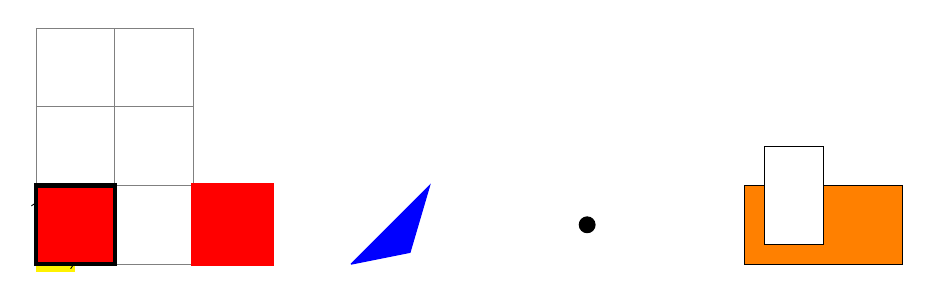
\begin{tikzpicture}[scale=1]
\draw[help lines] (0,0) grid (2,3);
\draw [yellow, line width=6]
(0,0) -- (.5,0); 
\draw [<->] (0,0.8) -- (0,0) -- (0.5,0);
\draw[green, ultra thick, domain=0:0.5] plot (\x, {0.025+\x+\x*\x});
\draw [fill=red,ultra thick] (0,0) rectangle (1,1);
\draw [fill=red,ultra thick,red] (2,0) rectangle (3,1);
\draw [blue, fill=blue] (4,0) -- (5,1) -- (4.75,0.15) -- (4,0);
\draw [fill] (7,0.5) circle [radius=0.1];
\draw [fill=orange] (9,0) rectangle (11,1);
\draw [fill=white] (9.25,0.25) rectangle (10,1.5);
\end{tikzpicture}

\begin{tikzpicture}
\path [fill=gray] (0,0) rectangle (1.5,1);
\draw [fill=yellow] (2,0) rectangle (3.5,1);
\end{tikzpicture}
\begin{tikzpicture}
\draw [thick, <->] (0,3) -- (0,1) -- (2,1);
\node at (2,2) {yes};
\end{tikzpicture}
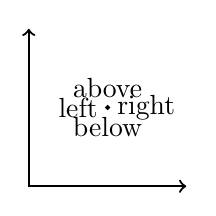
\begin{tikzpicture}
\draw [thick, <->] (0,2) -- (0,0) -- (2,0);
\draw[fill] (1,1) circle [radius=0.025];
\node [below] at (1,1) {below};
\node [above] at (1,1) {above};
\node [left] at (1,1) {left};
\node [right] at (1,1) {right};
\end{tikzpicture}
\begin{tikzpicture}[xscale=3, yscale=1.5]
\draw [thick, <->] (0,1) -- (0,0) -- (1,0);
\node [below right] at (1,0) {$x$};
\node [left] at (0,1) {$y$};
\draw[fill] (.4,.6) circle [radius=.5pt];
\node[above right] (.4,.6) {$A$};
\end{tikzpicture}
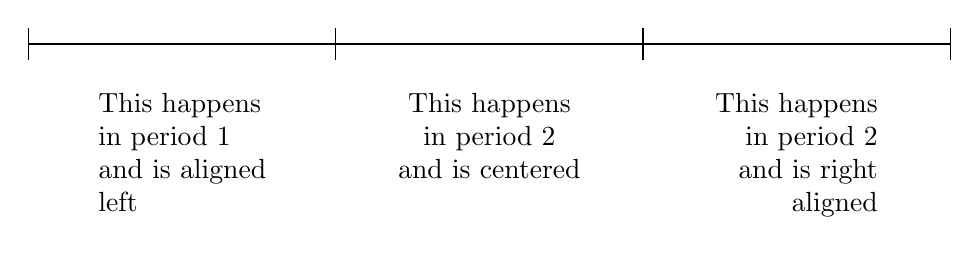
\begin{tikzpicture}[xscale=1.3]
\draw [thick] (0,0) -- (9,0);
\draw (0,-.2) -- (0, .2);
\draw (3,-.2) -- (3, .2);
\draw (6,-.2) -- (6, .2);
\draw (9,-.2) -- (9, .2);
\node[align=left, below] at (1.5,-.5)%
{This happens\\in period 1\\and is aligned\\ left};
\node[align=center, below] at (4.5,-.5)%
{This happens\\in period 2\\and is centered};
\node[align=right, below] at (7.5,-.5)%
{This happens\\in period 2\\and is right\\aligned};
\end{tikzpicture}
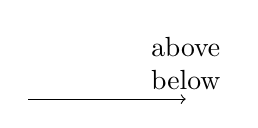
\begin{tikzpicture}
\draw [->] (0,0) -- (2,0);
\node [align=right,above] at (2,0) {above\\below};
\end{tikzpicture}
